\chapter[Understanding the Tiebreaking Strategies]{Understanding the Tiebreaking Strategies in High-Dimensional Search Spaces}

In this chapter, we investigate \emph{tie-breaking strategies} and \emph{plateau structure} for cost-optimal \astar search.
\astar is a standard search algorithm for finding an optimal cost path from an initial state $s$ to some goal
state $g \in G$ in a search space represented as a graph \cite{hart1968formal}.
It expands the nodes in best-first order of $f(n)$ up to $f^*$,
where $f(n)$ is a lower bound of the cost of the shortest path that contains a node $n$ and $f^*$ is
 the cost of the optimal path.
% 
In many combinatorial search problems, the size of the last layer $f(n)=f^*$ of the search, called a
 \emph{final plateau},
accounts for a significant fraction of the effective search space of \astar.  \refig{fig:plateau-noh}
(\refpage{fig:plateau-noh}) compares the number of states in this final plateau with $f(n) = f^*$ (y-axis)
vs. $f(n) \leq f^*$ (x-axis) for 1104 problem instances from the International Planning Competition (IPC1998-2011).
For many instances, a large fraction of the nodes in the effective search space have $f(n)=f^*$: The points
are located very close to the diagonal line ($x=y$), indicating that almost all states with $f(n) \leq f^*$ have cost
$f^*$.

\refig{fig:plateau-0} depicts this phenomenon conceptually.
% 
On the left, we show 
one natural  % avoiding ``naive'' here because we don't want to Frontier Search people to misunderstand and belive that we're calling them naive.
view of the search space that considers the space searched by \astar as
a large number of closed nodes with $f<f^*$, surrounded by
a thin layer of final plateau $f(n)=f^*$.  This intuitive view
accurately reflects the search spaces of some real-world problems such as 2D pathfinding on an explicit
graph.
% 
It has also served as a model for algorithms such as Frontier Search \cite{korf1999divide,korf2000divide},
which tries to reduce the memory requirement by discarding the information associated with states with $f<f^*$,
 an effective strategy when the number of such states accounts for a large fraction of the memory usage.
 
However, for many other classes of combinatorial search problems, e.g., the IPC Planning Competition Benchmarks, 
the figure on the right is a more accurate depiction -- here, the  search space has a large plateau for $f=f^*$.
In fact, Iterative Deepening approaches \cite{korf1985depth} assume this type of search space
where this final frontier is quite large and the overhead of re-evaluating $f<f^*$ is limited.
Classical planning problems in the IPC benchmark set are clearly the instances of such combinatorial search problems.

\todo*{The fact that the last layer of search dominates the search was
 the motivation for Frontier Search and its numerous variants, so the
 SoCS community has been well aware of this --- SoCS community considers
 the opposite. Frontier search would not gain advantage in the planning
 domains because the number of nodes being forgotten is low compared to
 the size of the plateau.}

\begin{figure}[htbp]
  \centering
  \includegraphics[width=\linewidth]{tables/aaai16-frontier/aaai16prelim3/lmcut_frontier_noh-front.pdf}
 \caption{
 The number of nodes with $f=f^*$ (y-axis) compared to the
 total number of nodes in the search space (x-axis) with $f\leq f^*$ on 1104 IPC benchmark problems.
 This experiment uses a modified Fast Downward with \lmcut which 
 continues the search within the current $f$ after any cost-optimal solution is found.
 This effectively generates all nodes with cost $f^*$.
  }
 \label{fig:plateau-noh}
\end{figure}

\begin{figure}[htbp]
  \centering
  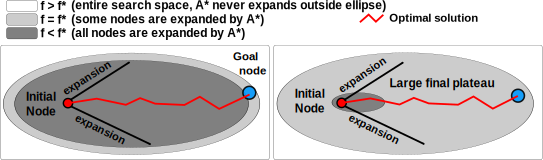
\includegraphics[width=\linewidth]{img/astar/plateau-0.pdf}
% \caption{(Left) Naive understanding of the search space of \astar, which only holds for some limited domains. (Right) The reality of search spaces of combinatorial problems. The plateau containing the cost-optimal goals ($f=f^*$) is large, and it even accounts for most of the search effort required by \astar.
 \caption{(Left) One possible class of search space which is dominated by the states with cost $f<f^*$. (Right) This paper focuses on another class of search space, where the plateau containing the cost-optimal goals ($f=f^*$) is large, and it even accounts for most of the search effort required by \astar. % reworded to avoid offending all the SoCS people.
  }
 \label{fig:plateau-0}
\end{figure}

For the majority of such IPC problem domains where
the last layer ($f(n)=f^*$) accounts for a significant fraction of the effective search space, a
\emph{tie-breaking strategy}, which determines which node to expand among nodes with the same $f$-cost,
can have a significant impact on the performance of \astar.
It is widely believed that among nodes with the same $f$-cost,
ties should be broken according to $h(n)$, i.e.,
nodes with smaller $h$-values should be expanded first.  While this is a
useful rule of thumb in many domains, it turns out that tie-breaking
requires more careful consideration, particularly for problems where
most or all of the nodes in the last layer have the same $h$-value.

We empirically evaluate the existing, commonly used, standard
tie-breaking strategies for \astar (\refsec{sec:eval-common-strategies}).
We show that:

\begin{enumerate}
 \item In the experiments on IPC domains,
       A Last-In-First-Out (\lifo) criterion tends to be more efficient
       than a First-In-First-Out (\fifo) criterion.
 \item Tie-breaking according to the heuristic value $h$, which
       is frequently mentioned in the heuristic search literature, has little
       impact on the performance as long as \lifo default criterion is used 
       --  in other words, a \lifo tie-breaking policy is sufficient for most IPC domains.
 \item There are significant performance differences among tie-breaking strategies
       when domains include 0-cost actions. This is true even when $h$-based tie-breaking is used.
\end{enumerate}
